\documentclass[letterpaper,10pt]{article}

% ============================================
% PACKAGES
% ============================================
\usepackage[empty]{fullpage}
\usepackage[usenames,dvipsnames]{xcolor}
\usepackage{enumitem}
\usepackage[hidelinks]{hyperref}
\usepackage{tabularx}
\usepackage{fontawesome5}
\usepackage{tikz}
\usepackage{geometry}
\usepackage[T1]{fontenc}
\usepackage{montserrat}
\usepackage{opensans}

\usetikzlibrary{shapes.geometric}

% ============================================
% GEOMETRY
% ============================================
\geometry{
    left=0.5in,
    right=0.4in,
    top=0.3in,
    bottom=0.2in
}

% Google Colors
\definecolor{GoogleBlue}{HTML}{4285F4}
\definecolor{GoogleRed}{HTML}{EA4335}
\definecolor{GoogleYellow}{HTML}{FBBC05}
\definecolor{GoogleGreen}{HTML}{34A853}
\definecolor{GoogleGray}{HTML}{5F6368}
\definecolor{GoogleLightGray}{HTML}{DADCE0}
\definecolor{LinkBlue}{HTML}{1A0DAB}
\definecolor{UrlGreen}{HTML}{1E8E3E}
\definecolor{TextBlack}{HTML}{202124}
\definecolor{SubtleGray}{HTML}{70757A}
\definecolor{PanelBorder}{HTML}{DFE1E5}
\definecolor{AIOverviewBg}{HTML}{EDF4FC}
\definecolor{AIPurple}{HTML}{7B61FF}

\pagestyle{empty}
\setlength{\parindent}{0pt}
\setlength{\parskip}{0pt}
\renewcommand{\familydefault}{\sfdefault}

% ATS-friendly PDF metadata
\hypersetup{
    pdftitle={Ayush Singh - Software Engineer Resume},
    pdfauthor={Ayush Singh},
    pdfsubject={Software Engineer III at Google},
    pdfkeywords={Software Engineer, Google, Distributed Systems, Backend Development, C++, Java, Go, TypeScript, Python, Scala, System Design, Technical Leadership, CI/CD}
}

% ============================================
% CUSTOM COMMANDS
% ============================================
\newcommand{\GoogleLogoSmall}{%
    \fontfamily{Montserrat-TOsF}\selectfont\fontsize{20}{22}\selectfont\bfseries%
    {\color{GoogleBlue}G}{\color{GoogleRed}o}{\color{GoogleYellow}o}{\color{GoogleBlue}g}{\color{GoogleGreen}l}{\color{GoogleRed}e}%
}

% ============================================
% DOCUMENT
% ============================================
\begin{document}

% ============================================
% HEADER
% ============================================
\begin{tabular}{@{}l@{\hspace{14pt}}l@{}}
\GoogleLogoSmall &
\begin{tikzpicture}[baseline=-3pt]
    \node[draw=GoogleLightGray, rounded corners=16pt, minimum height=28pt, text width=4.4in, inner xsep=10pt, inner ysep=0pt, fill=white, line width=0.5pt] {%
        {\small\color{GoogleGray}\faSearch}~~{\fontfamily{fos}\selectfont\small Ayush Singh - Distributed Systems Engineer}%
        \hfill{\small\color{GoogleGray}\faTimes}~~{\small\color{GoogleBlue}\faMicrophone}%
    };
\end{tikzpicture}
\end{tabular}

\vspace{4pt}
{\fontfamily{fos}\selectfont\footnotesize\color{SubtleGray}%
{\color{GoogleBlue}\underline{All}}~\hspace{12pt}%
\href{https://linkedin.com/in/iu-sh}{\faLinkedin~LinkedIn}~\hspace{12pt}%
\href{https://github.com/iu-sh}{\faGithub~GitHub}~\hspace{12pt}%
\href{https://ayushsingh.is-a.dev}{\faGlobe~Website}~\hspace{12pt}%
\href{mailto:apparently.ayush@gmail.com}{\faEnvelope~Email}%
}
\vspace{2pt}
{\color{GoogleLightGray}\hrule height 0.4pt}
\vspace{5pt}

% ============================================
% TWO COLUMNS
% ============================================
\begin{minipage}[t]{0.58\textwidth}

% AI Overview
\colorbox{AIOverviewBg}{%
\begin{minipage}[t]{0.96\linewidth}
\vspace{4pt}
{\color{AIPurple}\footnotesize\faRobot}~{\fontfamily{Montserrat-TOsF}\selectfont\footnotesize\bfseries\color{TextBlack}AI Overview}\\[3pt]
{\fontfamily{fos}\selectfont\small\color{TextBlack}%
\textbf{TL;DR: Swiss Army Knife} -- Distributed Systems, Core C++/Java Infrastructure, Distributed Storage. Google Munich (L4). Defaulted architecture across \textbf{$\sim$5,200 prod nodes}, built storage for \textbf{100K+ services}, delivered \textbf{\$2.5M+/quarter savings}, \textbf{promoted in 15 months}, and awarded \textbf{VP Spot Bonus}.%
}
\vspace{4pt}
\end{minipage}%
}

\vspace{6pt}

% EXPERIENCE
{\fontfamily{Montserrat-TOsF}\selectfont\normalsize\bfseries\color{TextBlack}Experience}
\vspace{4pt}

% Google Munich
{\fontfamily{fos}\selectfont\footnotesize\color{UrlGreen}careers.google.com › munich › swe-iii}\\[-2pt]
{\fontfamily{fos}\selectfont\color{LinkBlue}\normalsize\bfseries Software Engineer III} {\normalsize· \textbf{Google, Munich}}\\[1pt]
{\fontfamily{fos}\selectfont\footnotesize\color{SubtleGray}November 2024 -- Present | C++, Java, Kotlin, gRPC}\\[2pt]
{\fontfamily{fos}\selectfont\small\color{TextBlack}%
• Shipped global request-path processors into \textbf{Google's core Java backend framework} (powering all Google products) and \textbf{core C++ Search serving engine}, serving billions of daily users.\\[1pt]
• Authored org-wide microservice architecture defaulted across \textbf{$\sim$5,200 production server nodes} (210+ modules across Search, YouTube, Maps), cutting signal-processing complexity by \textbf{40\%} and retiring \textbf{1,300+ legacy LOC}.\\[1pt]
• Built parallel stream shadow-diffing across \textbf{YouTube, Play, Search \& Payments} (\textbf{100\% live cut-over parity}) and migrated \textbf{7 identity pipelines} to distributed batch compute.\\[1pt]
• Led end-to-end \textbf{UK Online Safety Act} and \textbf{US AppStore Age Verification} distributed backend launches across Web, Android, and iOS in 4 weeks across 5+ teams (\textbf{VP of Engineering Spot Bonus}).%
}

\vspace{5pt}

% Google India
{\fontfamily{fos}\selectfont\footnotesize\color{UrlGreen}careers.google.com › india › swe-iii}\\[-2pt]
{\fontfamily{fos}\selectfont\color{LinkBlue}\normalsize\bfseries Software Engineer II $\rightarrow$ III} {\normalsize· \textbf{Google, India}}\\[1pt]
{\fontfamily{fos}\selectfont\footnotesize\color{SubtleGray}July 2022 -- November 2024 | C++, Go, FUSE, Paxos, OpenTelemetry}\\[2pt]
{\fontfamily{fos}\selectfont\small\color{TextBlack}%
• Engineered fault-tolerant storage and replication for \textbf{Google's internal HDFS-like distributed file system}, optimizing binary delivery across \textbf{100,000+ internal services}.\\[1pt]
• Shipped server-side admission control, bounded semaphore RPC concurrency limiting in the \textbf{FUSE client}, and migrated distributed snapshot locks off \textbf{Paxos lock services}.\\[1pt]
• Architected an automated \textbf{SLA/SLO compliance \& observability platform} correlating distributed traces and metrics, saving \textbf{\$2.5M+ per quarter}.\\[1pt]
• Co-architected a real-time \textbf{OpenTelemetry} collector over \textbf{gRPC-Web} and encrypted \textbf{Go asset gateway}; led Chrome 3P cookie deprecation analysis (\textbf{CEO-level approval}) and earned \textbf{fast-track promotion to L4 in 15 months}.%
}

\vspace{5pt}

% Komprise
{\fontfamily{fos}\selectfont\footnotesize\color{UrlGreen}komprise.com › careers}\\[-2pt]
{\fontfamily{fos}\selectfont\color{LinkBlue}\normalsize\bfseries Software Engineer Intern} {\normalsize· \textbf{Komprise}}~{\footnotesize\color{SubtleGray}| Jan -- Jun 2022}\\[1pt]
{\fontfamily{fos}\selectfont\small\color{TextBlack}%
• Developed automated testing framework enabling parallel execution and proactive bug detection.\\[1pt]
• Optimized Build Verification Test suite through multi-threading, achieving \textbf{87.5\% reduction} in execution time.%
}

\vspace{5pt}

% Accenture
{\fontfamily{fos}\selectfont\footnotesize\color{UrlGreen}accenture.com › careers}\\[-2pt]
{\fontfamily{fos}\selectfont\color{LinkBlue}\normalsize\bfseries Data Engineer Intern} {\normalsize· \textbf{Accenture}}~{\footnotesize\color{SubtleGray}| May -- Jul 2021}\\[1pt]
{\fontfamily{fos}\selectfont\small\color{TextBlack}%
• Architected end-to-end Business Intelligence dashboard for E-Commerce analytics with AWS S3 to Snowflake data pipeline.\\[1pt]
• Developed NLP-powered conversational AI chatbot for automated data insights extraction.%
}

\vspace{5pt}

% Tookitaki
{\fontfamily{fos}\selectfont\footnotesize\color{UrlGreen}tookitaki.com › careers}\\[-2pt]
{\fontfamily{fos}\selectfont\color{LinkBlue}\normalsize\bfseries Software Engineer Intern} {\normalsize· \textbf{Tookitaki, Singapore}}~{\footnotesize\color{SubtleGray}| Oct 2020 -- Jan 2021}\\[1pt]
{\fontfamily{fos}\selectfont\small\color{TextBlack}%
• Engineered real-time streaming pipeline using Spark Structured-Streaming and ActiveMQ. Reduced message latency by \textbf{94\%} (0.85s → <0.05s).\\[1pt]
• Implemented custom JMS-Client with fault-tolerant message recovery mechanism.%
}

\end{minipage}%
\hfill%
% ============================================
% RIGHT PANEL
% ============================================
\begin{minipage}[t]{0.39\textwidth}

\fboxsep=6pt
\fboxrule=0.5pt
\fcolorbox{PanelBorder}{white}{%
\begin{minipage}[t]{0.90\linewidth}

{\fontfamily{Montserrat-TOsF}\selectfont\Large\bfseries\color{TextBlack}Ayush Singh}\\[1pt]
{\fontfamily{fos}\selectfont\small\color{SubtleGray}Software Engineer III (L4) @ Google, Munich}

\vspace{4pt}{\color{GoogleLightGray}\rule{\linewidth}{0.3pt}}\vspace{4pt}

{\fontfamily{Montserrat-TOsF}\selectfont\small\bfseries\color{TextBlack}About}\\[2pt]
{\fontfamily{fos}\selectfont\footnotesize\color{TextBlack}%
Software Engineer III at Google Munich specializing in planet-scale distributed systems, core C++/Java/Go infrastructure, and distributed storage. 4+ years driving high-impact systems.%
}

\vspace{4pt}

{\fontfamily{fos}\selectfont\footnotesize%
\textbf{\color{SubtleGray}Location:}~{\color{TextBlack}Munich, Germany}\\[1pt]
\textbf{\color{SubtleGray}Experience:}~{\color{TextBlack}4+ years}\\[1pt]
\textbf{\color{SubtleGray}Education:}~{\color{LinkBlue}\href{https://www.nita.ac.in/}{NIT Agartala}}\\[1pt]
\textbf{\color{SubtleGray}Degree:}~{\color{TextBlack}B.Tech (EE), 9.32/10}%
}

\vspace{4pt}{\color{GoogleLightGray}\rule{\linewidth}{0.3pt}}\vspace{4pt}

{\fontfamily{Montserrat-TOsF}\selectfont\small\bfseries\color{TextBlack}Contact}\\[2pt]
{\fontfamily{fos}\selectfont\footnotesize%
\faPhone*~+49 1735 34 8915\\[1pt]
\faEnvelope~{\color{LinkBlue}\href{mailto:apparently.ayush@gmail.com}{apparently.ayush@gmail.com}}\\[1pt]
\faLinkedin~{\color{LinkBlue}\href{https://linkedin.com/in/iu-sh}{linkedin.com/in/iu-sh}}\\[1pt]
\faGlobe~{\color{LinkBlue}\href{https://ayushsingh.is-a.dev}{ayushsingh.is-a.dev}}%
}

\vspace{4pt}{\color{GoogleLightGray}\rule{\linewidth}{0.3pt}}\vspace{4pt}

{\fontfamily{Montserrat-TOsF}\selectfont\small\bfseries\color{TextBlack}Technical Skills}\\[2pt]
{\fontfamily{fos}\selectfont\footnotesize\color{TextBlack}%
\textbf{Languages:} C++, Java, Go, TypeScript, Scala, Python, Kotlin\\[1pt]
\textbf{Systems:} gRPC, Protobuf, HDFS/FUSE, Paxos, Spark, Kafka\\[1pt]
\textbf{Storage \& DB:} Spanner, Snowflake, Redis, PostgreSQL\\[1pt]
\textbf{Cloud \& Tools:} Kubernetes, Docker, OpenTelemetry, GCP, AWS%
}

\vspace{4pt}{\color{GoogleLightGray}\rule{\linewidth}{0.3pt}}\vspace{4pt}

{\fontfamily{Montserrat-TOsF}\selectfont\small\bfseries\color{TextBlack}Achievements}\\[2pt]
{\fontfamily{fos}\selectfont\footnotesize\color{TextBlack}%
{\color{GoogleBlue}\faTrophy}~VP of Engineering Spot Bonus\\[1pt]
{\color{GoogleBlue}\faTrophy}~3$\times$ Google Readability (1,040+ CLs)\\[1pt]
{\color{GoogleBlue}\faTrophy}~7 Peer Bonuses at Google\\[1pt]
{\color{GoogleGreen}\faMedal}~Rank 1 GFG at NIT-A (\#72 Global)\\[1pt]
{\color{GoogleBlue}\faAward}~IASc Fellowship 2021 (1/11)\\[1pt]
{\color{GoogleGreen}\faUsers}~Founded Google DSC @ NIT-A%
}

\vspace{4pt}{\color{GoogleLightGray}\rule{\linewidth}{0.3pt}}\vspace{4pt}

{\fontfamily{Montserrat-TOsF}\selectfont\small\bfseries\color{TextBlack}Projects}\\[2pt]
{\fontfamily{fos}\selectfont\footnotesize\color{TextBlack}%
{\color{LinkBlue}\href{https://github.com/iu-sh/ytm_ai_host}{\textbf{YTM AI Host}}} -- Real-time (<100ms) AI Radio Jockey for YouTube Music \& Spotify (Gemini API, WebLLM/WebGPU)\\[1pt]
{\color{LinkBlue}\href{https://github.com/iu-sh/linkinJMS}{\textbf{LinkinJMS}}} -- High-performance Spark \& ActiveMQ connector (<50ms latency)\\[1pt]
{\color{LinkBlue}\href{https://youtu.be/0Fff2ncdbPo}{\textbf{Pika Robot}}} -- Autonomous navigation using Computer Vision (TensorFlow, OpenCV)%
}

\vspace{4pt}{\color{GoogleLightGray}\rule{\linewidth}{0.3pt}}\vspace{4pt}

{\fontfamily{Montserrat-TOsF}\selectfont\small\bfseries\color{TextBlack}Profiles}\\[2pt]
{\fontfamily{fos}\selectfont\footnotesize%
{\color{GoogleBlue}\faLinkedin}~{\color{LinkBlue}\href{https://linkedin.com/in/iu-sh}{LinkedIn}}~~%
{\color{TextBlack}\faGithub}~{\color{LinkBlue}\href{https://github.com/iu-sh}{GitHub}}~~%
{\color{GoogleBlue}\faGlobe}~{\color{LinkBlue}\href{https://ayushsingh.is-a.dev}{Portfolio}}%
}

\end{minipage}%
}

\end{minipage}

\end{document}
